\chapter{Diseño y funcionamiento final}
Luego de todo el desarrollo de la aplicación mostraré el diseño y funcionamiento final que tiene.

\section{Inicio de sesión y registro de usuario}
\begin{figure}[h]
    \centering
    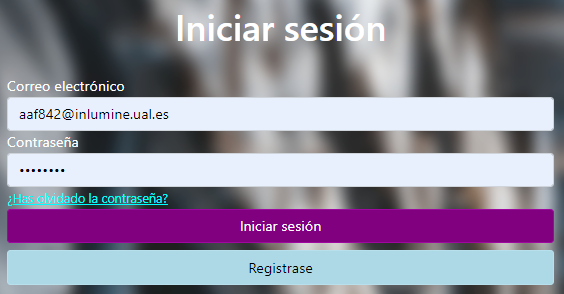
\includegraphics[scale=0.5,keepaspectratio]{../contruccion_aplicacion/design/login.png}
    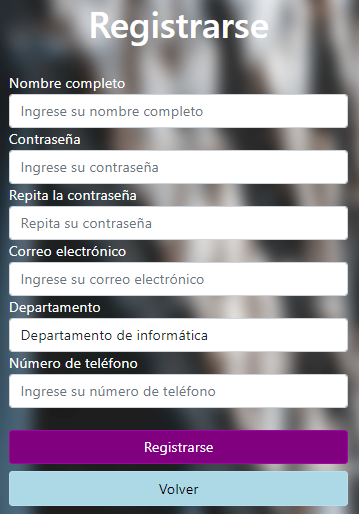
\includegraphics[scale=0.5,keepaspectratio]{../contruccion_aplicacion/design/register.png}
    \caption{A la izquierda el inicio de sesión y a la derecha el formulario de registro de usuario}\label{fig:register-and-login}
\end{figure}
En la figura \ref{fig:register-and-login} podemos ver cómo ha quedado el resultado final de nuestro registro e inicio de sesión de Inventarium. Dentro del cuadro de inicio de sesión se añade un enlace posibilitando una recuperación de la contraseña. Dicha recuperación tendría que ser facilitada por un técnico. En el complemento del trabajo de fin de grado junto a la implementación del gestor de correos completaremos la funcionalidad para que un usuario pueda recuperar sus credenciales.
\\Dentro del formulario de registro todos los campos deben ser rellenados de forma obligatoria. Además se han implementado comprobaciones para que estas variables cumplan con unas determinadas propiedades:
\begin{itemize}
    \item El campo del nombre completo debe contener más de ocho caracteres
    \item La contraseña debe tener más de ocho caracteres
    \item La entrada de ``Contraseña'' y la de ``Repita contraseña'' deben ser iguales
    \item El correo electrónico tiene que tener la extensión \textbf{@ual.es} o \textbf{@inlumine.ual.es}
    \item El apartado para ingresar el número de teléfono debe contener 9 dígitos exactos.
\end{itemize}

\section{Componentes principales}
Estos componentes reciben su nombre debido a que son la estructura principal de la aplicación. Son los átomos que conforman los distintos componentes.
\\Un ejemplo sería la figura \ref{fig:user-view}. En ella podemos ver cómo se muestran los campos que puede contener un usuario, el correo electrónico, el departamento al que pertenece, su número de teléfono y qué tipo de usuario es.
\begin{figure}[h]
    \centering
    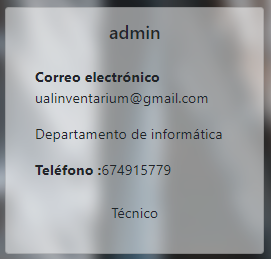
\includegraphics[scale=0.5,keepaspectratio]{../contruccion_aplicacion/design/user.png}
    \caption{Representación de un usuario en la aplicación}\label{fig:user-view}
\end{figure}
Este componente ha sido creado en base a uno principal con el cual también podríamos crear el de la figura \ref{fig:user-unit}.
\begin{figure}[h]
    \centering
    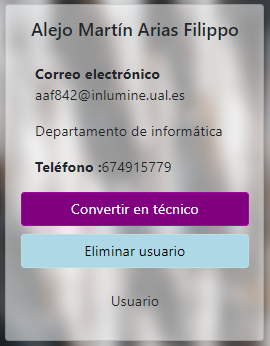
\includegraphics[scale=0.5,keepaspectratio]{../contruccion_aplicacion/design/user_unit.png}
    \caption{Representación de un usuario y posibles acciones sobre él en la aplicación}\label{fig:user-unit}
\end{figure}
¿Qué objetivo pretendo conseguir con esta diferenciación? En la modularización del código, es decir, en una separación entre visualización y acciones posibles sobre el objeto.
\\Es decir, esta vista donde se proyecta la visualización del usuario podemos ponerla en varias secciones del código pero, dónde podemos modificar su campos. No se pretende posibilitar la modificación de los campos en todos los sitios donde se llame al componente. Por ello creo el concepto de vistas unitarias.
\\En una vista unitaria se van a poder realizar todas las acciones posibles sobre un objeto. Esto nos ayudará a poder hacer una separación de permisos, dependiendo de si es un usuario o un técnico y a implementar modificaciones únicamente en un sitio en caso de realizar algún cambio. Por ejemplo el usuario de la figura \ref{fig:user-unit} es de la vista unitaria del usuario. Dentro de ella podemos realizar diferentes acciones como convertirlo en técnico o eliminarlo.
\\Esta diferencia de vistas nos permite crear relaciones que nos ayudarán en la gestión de la herramienta. Las vistas unitarias junto a sus respectivas relaciones son las siguientes:

\subsection{Usuario}
Dentro de un usuario dispondremos de un campo donde podremos acceder para visualizar sus préstamos. También podremos realizar diferentes acciones sobre él en caso de que seamos un usuario \textit{técnico}:
\begin{itemize}
    \item Dar de alta
    \item Eliminar
    \item Convertir en técnico
\end{itemize}

\subsection{Objeto}
En el objeto podremos acceder a un apartado donde veremos sus préstamos. También veremos el grupo de objetos al que pertenece y por último tendremos un campo donde podremos añadirle una configuración.
\\Para poder hacer una distinción de unos objetos de otros se les ha asociado a su nombre la id del elemento. Esto ayudará a los usuarios a distinguir posibles objetos que no tienen un código de inventario asociado a su nombre.
\\Podemos ver cómo nos queda la vista de los objetos en la figura \ref{fig:object-unit}.

\begin{figure}[h]
    \centering
    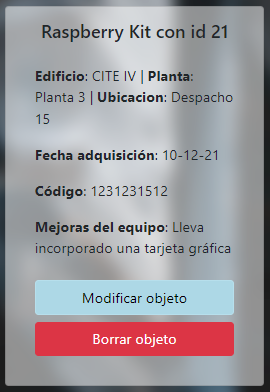
\includegraphics[scale=0.5,keepaspectratio]{../contruccion_aplicacion/design/object.png}
    \caption{Objeto y acciones que podemos hacer sobre él}\label{fig:object-unit}
\end{figure}

\subsection{Grupo de objetos}
Dentro de los grupos de objetos podremos visualizar los datos principales del grupo como puede ser la \textit{marca}, \textit{modelo} y \textit{nombre} y debajo de ella veremos los objetos que pertenecen a ese grupo.
\\Adicionalmente en el caso de que un objeto pertenezca a la categoría de \textit{kit} se mostrará un botón que pondrá \textit{¿Qué contiene el kit?} y que clicándolo nos mostrará los elementos del tipo \textit{objetokit} que contiene. Todo esto lo podemos ver en la figura \ref{fig:group-of-object-unit}.

\begin{figure}[h]
    \centering
    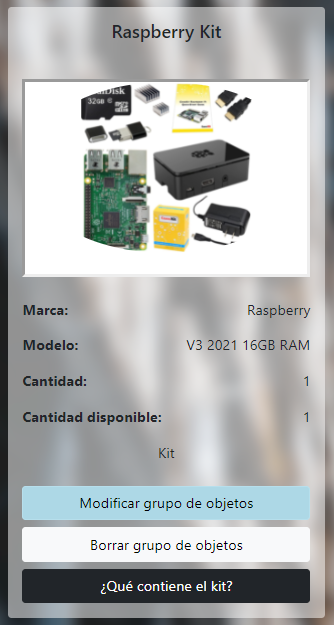
\includegraphics[scale=0.5,keepaspectratio]{../contruccion_aplicacion/design/group_of_object.png}
    \caption{Grupo de objeto y acciones que podemos hacer sobre él}\label{fig:group-of-object-unit}
\end{figure}


\subsection{Préstamos}
Al haber distintos campos de préstamos cada uno dispone de diferentes casos de usos. Estos son los de la figura \ref{fig:loans-diagram}.

\begin{figure}[h]
    \centering
    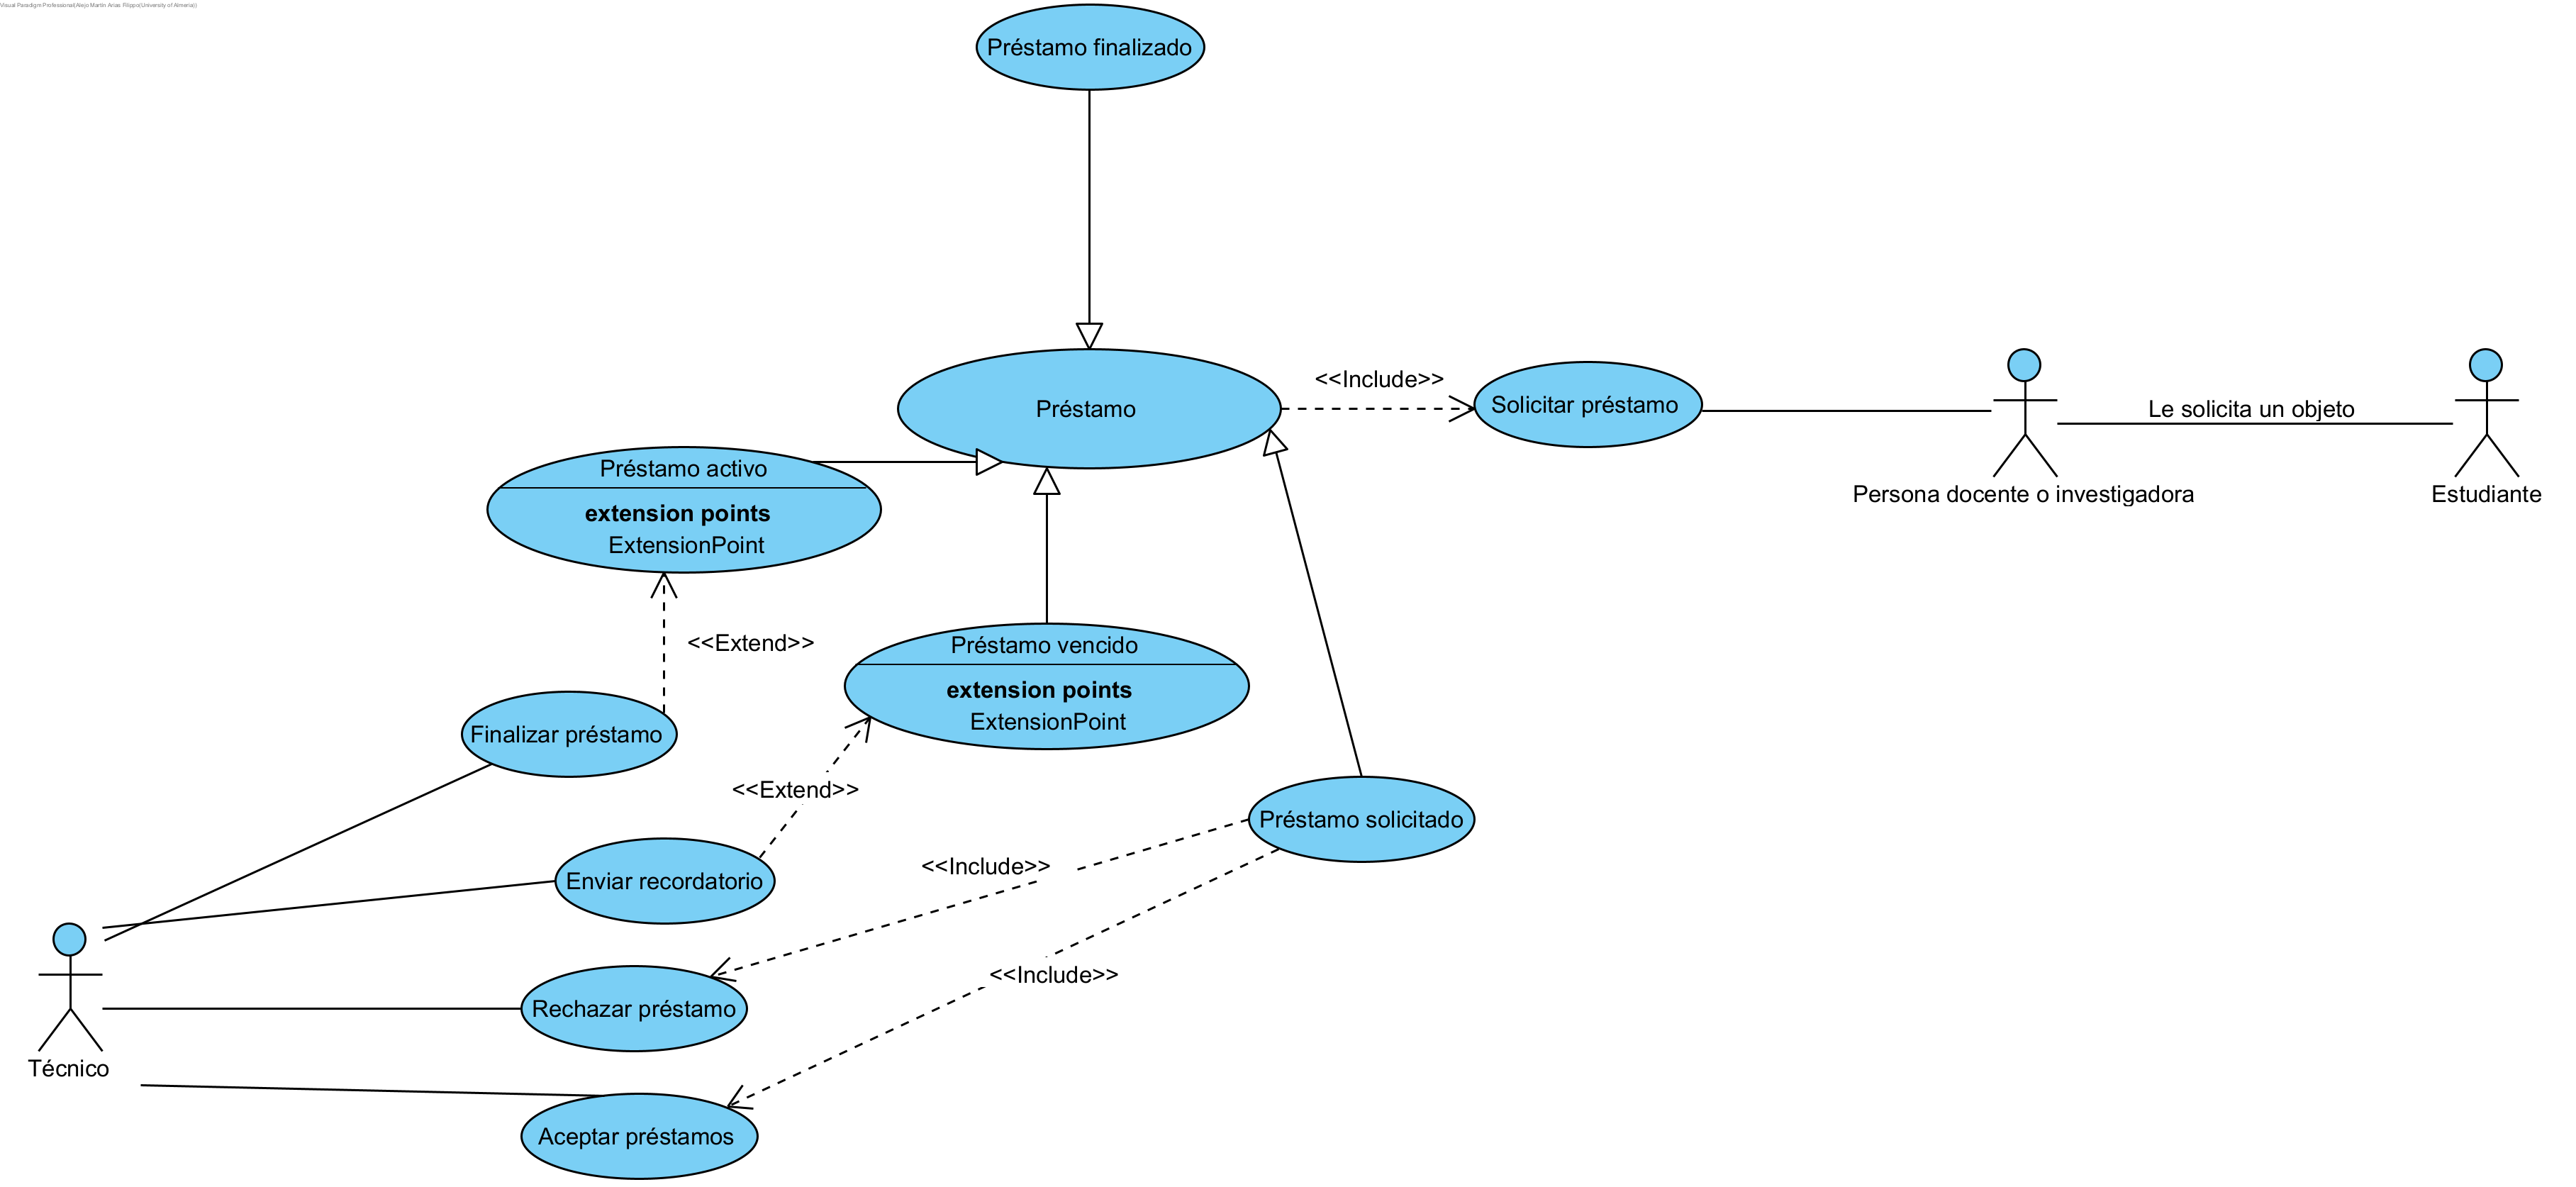
\includegraphics[scale=0.5,keepaspectratio]{../contruccion_aplicacion/prestamos-working.png}
    \caption{Funcionamiento y descomposición de préstamos}\label{fig:loans-diagram}
\end{figure}

\section{Componentes de procesos}
Habiendo visto los componentes principales que conforman la aplicación otro aspecto a destacar es el del desarrollo de los procesos. Distinguiremos cuatro tipos de procesos:
\begin{itemize}
    \item Proceso de creación de grupo de objetos y objetos
    \item Procesos de creación
    \item Procesos de modificación
    \item Proceso de creación, selección y eliminación de ubicaciones
\end{itemize}

\subsection{Proceso de creación de grupo de objetos y objetos}
Los procesos de creación de estos dos componentes tenía que llevar un aspecto de personalización debido a la interrelación que hay entre ellos.
\\Es decir, si un técnico quiere crear un objeto al pasar por este proceso va a saber si este ya ha sido creado con anterioridad para poder añadirlo al grupo de objetos.
\\Pero vayamos a ver la construcción y secuencia de vistas que ocurren en una creación de grupo de objetos y de objetos.
\subsubsection{Escoger el tipo}
El primer paso es escoger el tipo de objeto que deseas crear, tal como podemos ver en la figura \ref{fig:1-creation-o}

\begin{figure}[h]
    \centering
    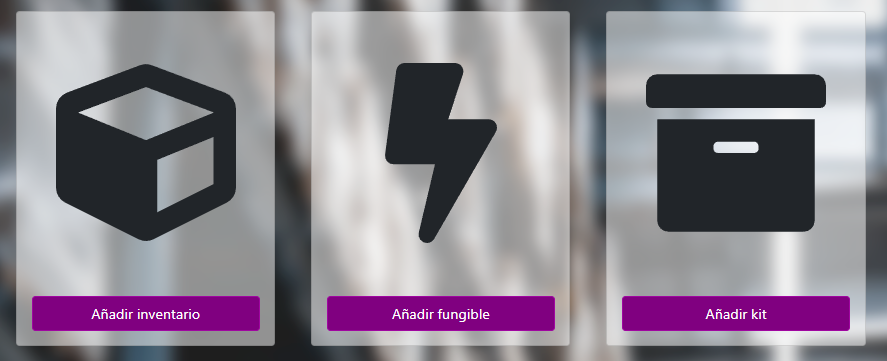
\includegraphics[scale=0.5,keepaspectratio]{../contruccion_aplicacion/design/add_object/01_add_object.png}
    \caption{Funcionamiento y descomposición de préstamos}\label{fig:1-creation-o}
\end{figure}

\subsubsection{Buscar o añadir el grupo de objeto}
Este proceso se encargará de que el usuario pueda ver si su grupo de objetos ya ha sido creado. En caso de que no lo sea puede pulsar en el botón de crear grupo de objetos para realizar una creación. Podemos observarlo en la figura \ref{fig:2-creation-o}.
\\En este ejemplo vamos a suponer que ha iniciado un proceso de creación de grupo de objetos.

\begin{figure}[h]
    \centering
    
\includegraphics[scale=0.5,keepaspectratio]{../contruccion_aplicacion/design/add_object/02_add_object.png}
    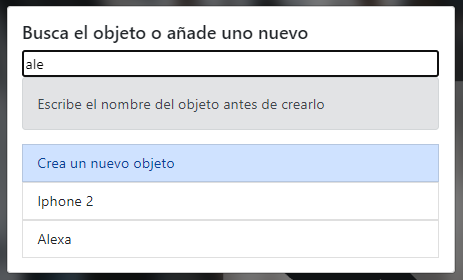
\includegraphics[scale=0.5,keepaspectratio]{../contruccion_aplicacion/design/add_object/03_add_object.png}
    \caption{Cuadros para iniciar la búsqueda de grupos de objetos}\label{fig:2-creation-o}
\end{figure}

\subsubsection{Añadir imagen y datos}
Uno de los requisitos obtenido en las entrevistas iniciales era que cada grupo de objeto tenía que ir asociado obligatoriamente con una imagen. Por lo que el subir una imagen es un proceso obligatorio en el proceso de creación de un grupo de objetos tal como vemos en la figura \ref{fig:3-creation-o}.

\begin{figure}[h]
    \centering
    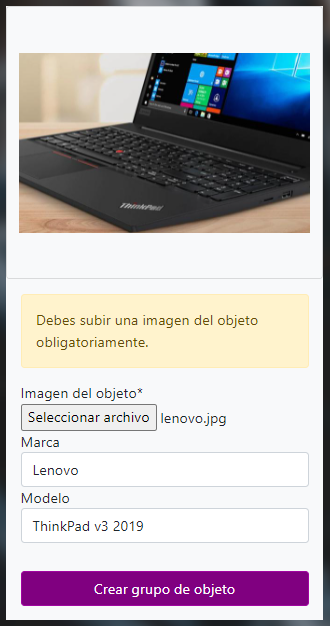
\includegraphics[scale=0.5,keepaspectratio]{../contruccion_aplicacion/design/add_object/04_add_object.png}
    \caption{Añadir imagen y datos al grupo de objetos}\label{fig:3-creation-o}
\end{figure}

\subsubsection{Creación de objetos}
Luego de haber generado nuestro grupo de objetos el sistema nos llevará a la ventana de adición de objetos. Esta vista es la misma a la que nos hubiera llevado en caso de que hubieramos seleccionado un grupo de objetos del cuadro de búsqueda.
\\Para empezar con la creación de elementos tendremos que elegir cuántos elementos querremos crear y dónde se ubicarán. El proceso de gestión de ubicaciones lo trataremos más adelante. De momento vemos el contenido de la figura \ref{fig:4-creation-o}.

\begin{figure}[h]
    \centering
    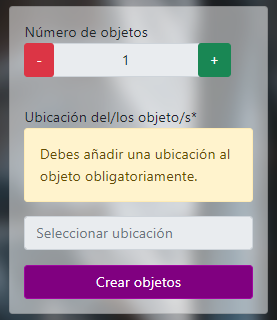
\includegraphics[scale=0.5,keepaspectratio]{../contruccion_aplicacion/design/add_object/05-add_object.png}
    \caption{Número de objetos y localización}\label{fig:4-creation-o}
\end{figure}

\subsubsection{Añadir datos a los objetos}
Al realizar el paso anterior nos llevará a una vista donde iremos añadiendo los datos de los objetos que queremos crear. En caso de que no queramos añadir los datos objeto por objeto hay un botón habilitado que realiza la creación de estos de forma automática pero sin la adición de los datos personalizados. Esto lo podemos ver en la figura \ref{fig:5-creation-o}.
\begin{figure}[h]
    \centering
    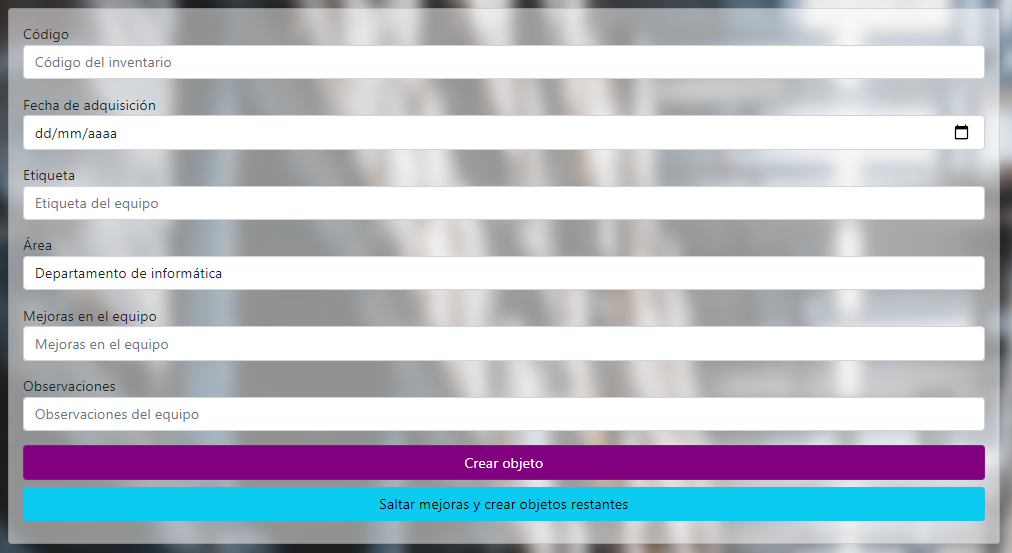
\includegraphics[scale=0.5,keepaspectratio]{../contruccion_aplicacion/design/add_object/07_add_object.png}
    \caption{Funcionamiento y descomposición de préstamos}\label{fig:5-creation-o}
\end{figure}

\subsection{Procesos de creación y modificación}
Estos procesos utilizan el mismo componente ya que la acción de modificación permite cambiar los mismos atributos que la acción de creación. Podemos ver un ejemplo en la figura \ref{fig:creation-and-modification}.
\begin{figure}[h]
    \centering
    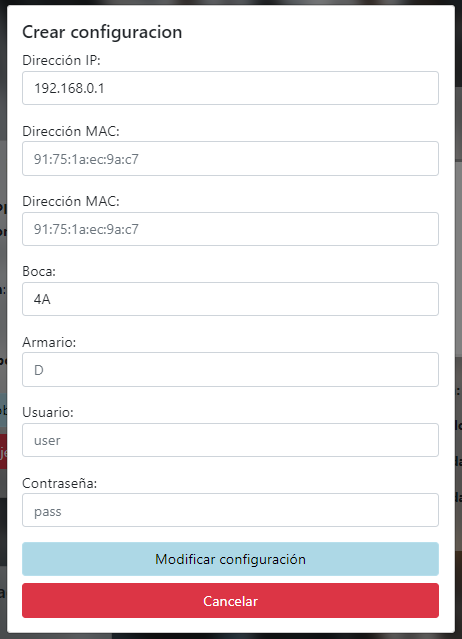
\includegraphics[scale=0.5,keepaspectratio]{../contruccion_aplicacion/design/configuration_form.png}
    \caption{Creación y modificación de elementos}\label{fig:creation-and-modification}
\end{figure}
\subsection{Proceso de creación, selección y eliminación de ubicaciones}
Una ubicación en la Universidad de Almería consta de tres atributos. Un edificio, una planta y una localización dentro de esa planta.
\\En base a estos distintos atributos haríamos el componente encargado de gestionar la ubicación de un objeto.
\\Este componente consta de tres etapas de selección la primera donde empiezas seleccionando el edificio, figura \ref{fig:1-loc-o}, luego podrás ver las plantas, figura \ref{fig:2-loc-o}, y luego las localizaciones dentro de esas plantas, figura \ref{fig:3-loc-o}.
\\En este proceso está presente en la parte superior una barra de búsqueda que también hace la función de creación. Es decir, en el caso de que no encuentres un edificio, escribes su nombre y a partir de ahí pasas a la siguiente etapa que es crear una planta para ese edificio. Hasta que no llegas a la etapa final de la creación de la localización esta ubicación no se genera.
\\Para poder eliminar las ubicaciones basta con seleccionar la localización que quieras eliminar y en caso de que esta esté enlazada con un objeto te pedirá que elimines dichos objetos o les cambies la ubicación. Si no lo haces, el sistema te impide eliminar la ubicación.
\begin{figure}[h]
    \centering
    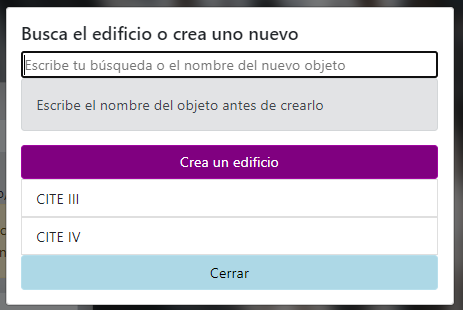
\includegraphics[scale=0.5,keepaspectratio]{../contruccion_aplicacion/design/add_object/add_location/06_01_add_location.png}
    \caption{Selección o creación del edificio}\label{fig:1-loc-o}
\end{figure}
\begin{figure}[h]
    \centering
    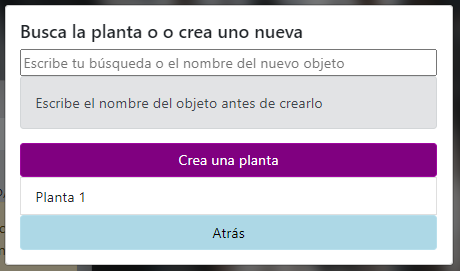
\includegraphics[scale=0.5,keepaspectratio]{../contruccion_aplicacion/design/add_object/add_location/06_02_add_location.png}
    \caption{Selección o creación de la planta}\label{fig:2-loc-o}
\end{figure}
\begin{figure}[h]
    \centering
    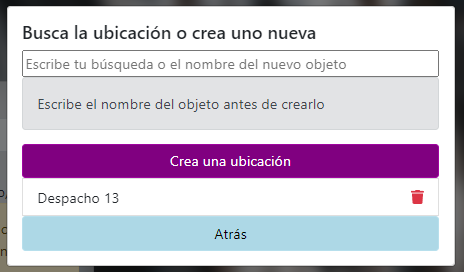
\includegraphics[scale=0.5,keepaspectratio]{../contruccion_aplicacion/design/add_object/add_location/06_03_add_location.png}
    \caption{Selección o creación de la ubicación}\label{fig:3-loc-o}
\end{figure}